\documentclass{article}

\usepackage{amsmath,amssymb}
\usepackage{hyperref}
\usepackage{amssymb}
\usepackage{graphicx}
\graphicspath{{../logos/}}


\begin{document}

\setlength{\tabcolsep}{5pt}
\begin{center} \begin{tabular}{cccc}
	
\includegraphics[height=43pt]{SAMF_logo.jpg} &
	
\includegraphics[height=43pt]{SAICA_logo.jpg} &
	
\includegraphics[height=43pt]{OM_Logo_Stacked_Vignette_on_White_RGB.jpg} &
	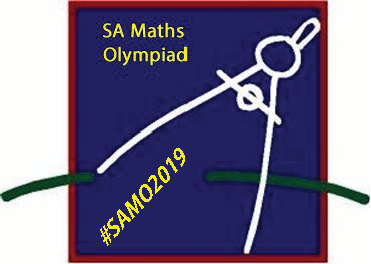
\includegraphics[height=43pt]{SAMO2019.png}
\end{tabular} \end{center}

\bigskip

\begin{center}
\textbf{\Large Another Senior Monthly Problem Set}
\\ \vspace{1em}
\textbf{\large Due: ~, ~ ~ 2020}
\end{center}


\begin{enumerate}

\bigskip
\item[1.] % 2015 Azerbaijan IMO TST, Q1
A set, $A=\{a_1, a_2, \cdots, a_n\}$, of distinct, positive integers is called ``powerful'' if
$$\prod_{i \neq j}^{}a_j \mid a_i^{2020}$$ 

for all $i \in \{1, 2, \cdots, n\}$. Find all $n \ge 3$ such that there exists a ``powerful'' set containing exactly $n$ elements.

\medskip
\item[2.] % All Russian Olympiad 2017, Grade 10, Q2 
Let $ABC$ be an acute angled isosceles triangle with $AB = AC$ and circumcentre $O$. Lines $BO$ and $CO$ intersect $AC$ and $AB$ at $D$ and $E$ respectively.
A straight line $l$ is drawn through $E$ parallel to $AC$. Prove that the line $l$ is tangent to the circumcircle of $\triangle DOC$.

\medskip
\item[3.] % 2017 Princeton University Maths Competition A4
Let the sequence $a_1$, $a_2$, $\cdots$ be defined by $a_n = 11a_{n - 1} - n$. Find the smallest possible value of $a_1$ such that $a_i > 0$ for all $i \in \mathbb{N}$.

\medskip
\item[4.] % China Southeast Math Olympiad 2014, Q2
There are $n \ge 4$ people at a fencing competition. Each player plays against every other player exactly once, and
there are no draws. The organisers decide that the competition is representative if they can find $4$ people: $a_1$,
$a_2$, $a_3$ and $a_4$, such that $a_i$ beats $a_j$ whenever $i < j$. Find the smallest value $n$ such that the
competition will always be representative.

\medskip
\item[5.] % 2011 Japan Mathematical Olympiad Finals Problem 5
Given some $4$ points in the plane, one can construct $4$ different triangles with vertices amongst the $4$ points. If the inscribed circles
of these $4$ triangles all have the same radius, show that the $4$ triangles are congruent. 

\medskip
\item[6.] % 

\medskip
\item[7.] % 

\medskip
\item[8.] % 

\end{enumerate}

\vfill
\textbf{\Large Email submission guidelines}
\begin{itemize}
	\item Email your solutions to \href{mailto:samf.training.assignments@gmail.com}{\texttt{samf.training.assignments@gmail.com}}.
	\item In the subject of your email, include your name and the level of the assignment (Beginner, Intermediate or Senior).
	\item Submit each question in a separate PDF file (with multiple pages if necessary), with your name and the question number written on each page.
	\item If you take photographs of your work, use a document scanner such as Office Lens to convert to PDF.
	\item If you have multiple PDF files for a question, combine them using software such as PDFsam.
\end{itemize}

\end{document}
